\documentclass[11pt,tikz,border=3.14mm]{standalone}
\usepackage{xcolor}
\definecolor{r1}{HTML}{FF8674}
\definecolor{b1}{HTML}{17ABDD}
\definecolor{p1}{HTML}{D4B6D6}
\definecolor{g1}{HTML}{70E2CB}
\definecolor{o1}{HTML}{DFA743}

\usepackage{mathptmx}
\usepackage{BOONDOX-cal} %使用花体emf
\newcommand\EMF{\mathcal{E}} %\varepsilon}
\usepackage[outline]{contour} % glow around text
\contourlength{1.5pt}


\usepackage[european]{circuitikz}
\tikzstyle{thick R}=[R, color=b1,l=$R$] %欧洲风格的电阻就是空心的,因此没有办法填充颜色
\tikzstyle{EMF}=[battery1,l=$\EMF$]
\tikzstyle{loop}=[-stealth,r1]
\tikzstyle{loop label}=[r1,fill=white,scale=0.8,inner sep=1]

\begin{document}
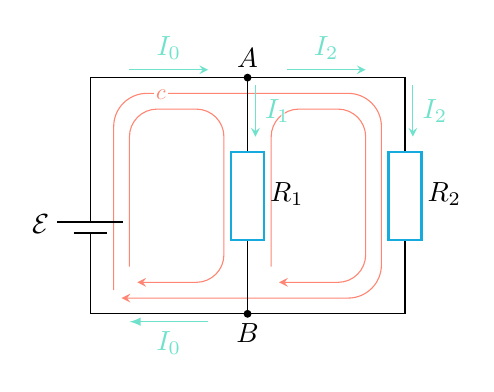
\begin{tikzpicture}
  \draw[rounded corners=12,loop] (0.3,0.3) |- (3.7,2.8) |- (0.4,0.2);
  \draw[rounded corners=10,loop] (0.5,0.6) |- (1.7,2.6) |- (0.6,0.4);
  \draw[rounded corners=10,loop] (2.3,0.6) |- (3.5,2.6) |- (2.4,0.4);
  \fill[black] (2,3) circle (0.05) node[above] {$A$};
  \fill[black] (2,0) circle (0.05) node[below] {$B$};
  \draw (0,0) to[EMF,invert] (0,2.2)
              -- (0,3) coordinate (I0) --++ (2,0) coordinate (I1)
              to[thick R,l=$R_1$] (2,0) coordinate (IF) -- (0,0);
  \draw (2,3) --++ (2,0) coordinate (I2)
              to[thick R,l=$R_2$] (4,0) -- (0,0);
  \draw[-stealth,g1] (I0)++(0.5, 0.1) --++ (1,0) node[midway,above] {$I_0$};
  \draw[-stealth,g1] (I1)++(0.1,-0.1) --++ (0,-0.65) node[midway,right] {\contour{white}{$I_1$}};
  \draw[-stealth,g1] (I1)++(0.5, 0.1) --++ (1,0) node[midway,above] {$I_2$};
  \draw[-stealth,g1] (I2)++(0.1,-0.1) --++ (0,-0.65) node[midway,right] {$I_2$};
  \draw[-latex,g1] (IF)++(-0.5,-0.1) --++ (-1,0) node[midway,below] {$I_0$};
  \node[loop label] at (0.90,2.78) {$c$};
  % \node[loop label] at (1.12,2.62) {$a$};
  % \node[loop label] at (2.92,2.62) {$b$};
\end{tikzpicture}
\end{document}